% Editable source for result.pdf, written by make_figures.py from
% run_github_38786433493/panel/result.json. Ratios with 95% bootstrap intervals over targets (or blocks);
% log2 axis; dashed line = parity.
\documentclass[tikz,border=6pt]{standalone}
\usepackage[T1]{fontenc}
\begin{document}
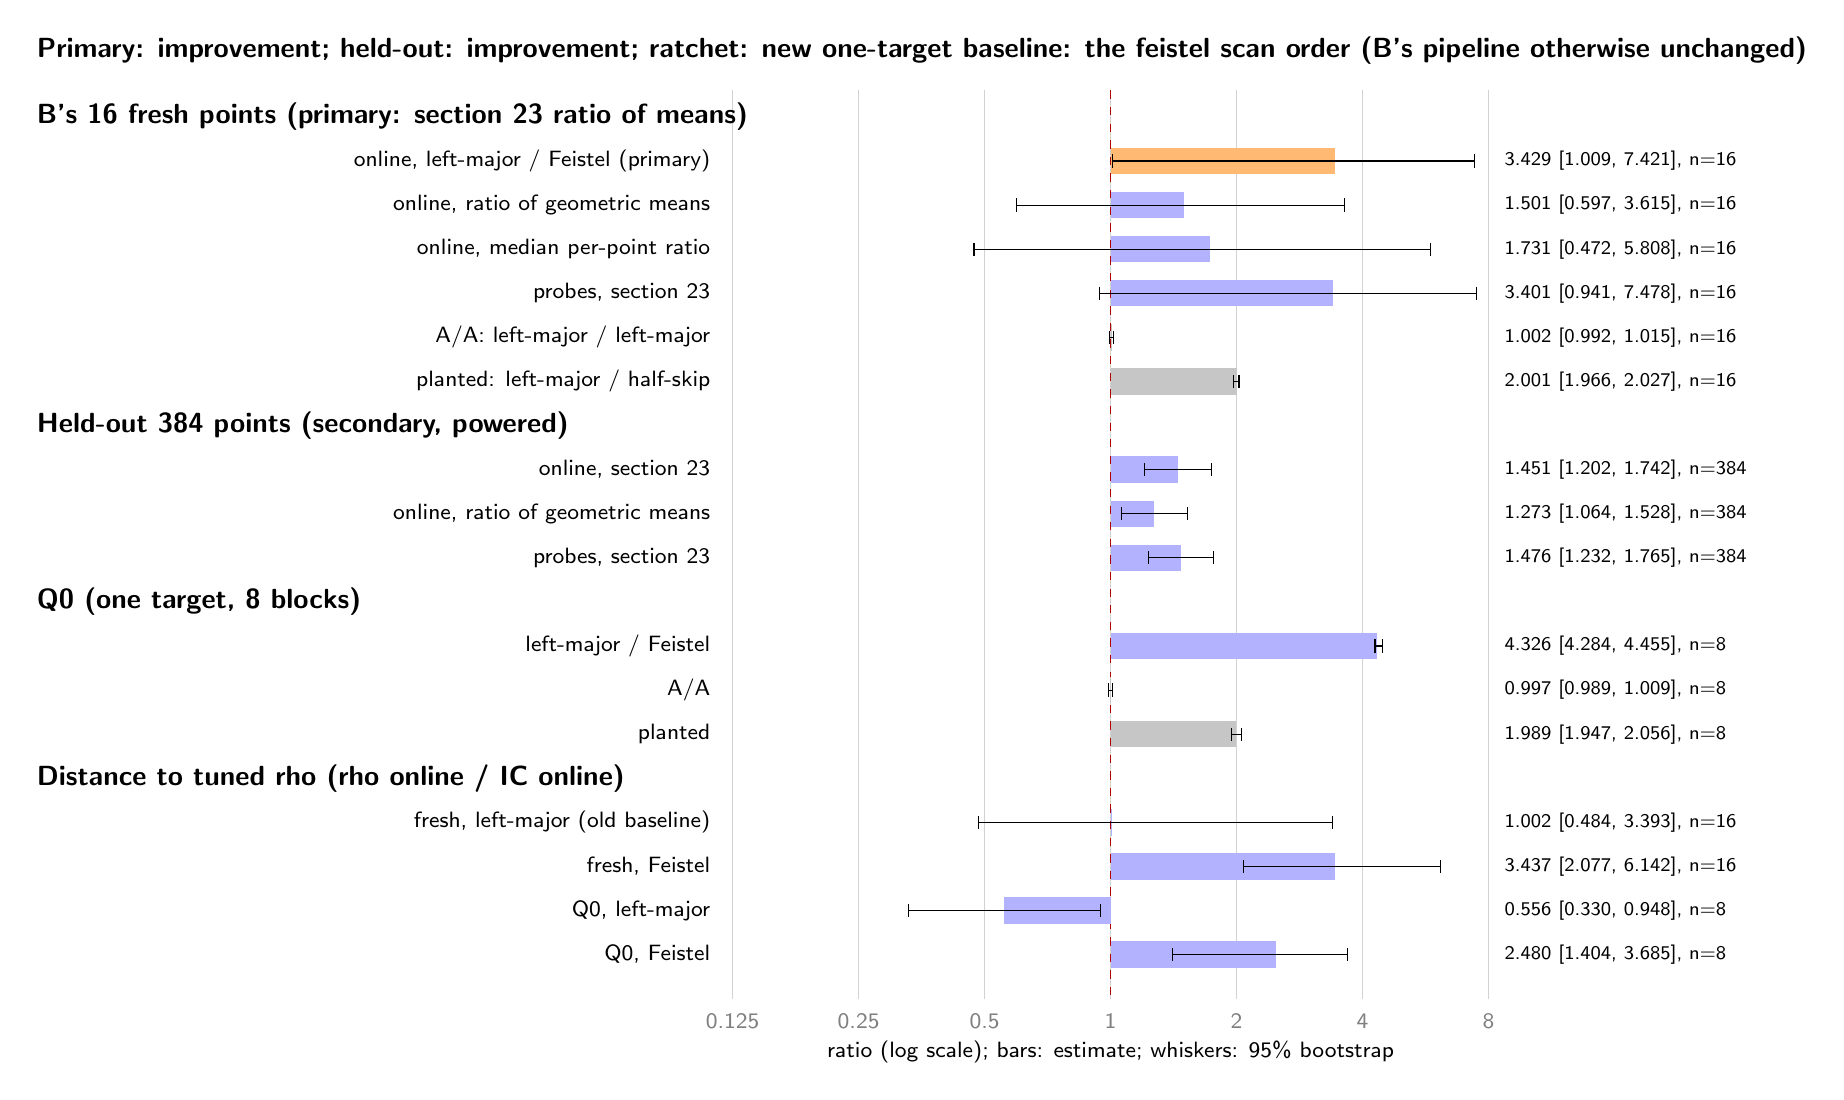
\begin{tikzpicture}[font=\sffamily\footnotesize,x=16mm,y=-5.6mm]
\draw[gray!35] (-3.0000,-0.6) -- (-3.0000,20); \node[gray] at (-3.0000,20.5) {0.125};
\draw[gray!35] (-2.0000,-0.6) -- (-2.0000,20); \node[gray] at (-2.0000,20.5) {0.25};
\draw[gray!35] (-1.0000,-0.6) -- (-1.0000,20); \node[gray] at (-1.0000,20.5) {0.5};
\draw[gray!35] (0.0000,-0.6) -- (0.0000,20); \node[gray] at (0.0000,20.5) {1};
\draw[gray!35] (1.0000,-0.6) -- (1.0000,20); \node[gray] at (1.0000,20.5) {2};
\draw[gray!35] (2.0000,-0.6) -- (2.0000,20); \node[gray] at (2.0000,20.5) {4};
\draw[gray!35] (3.0000,-0.6) -- (3.0000,20); \node[gray] at (3.0000,20.5) {8};
\draw[red!70!black,dashed] (0,-0.6) -- (0,20);
\node at (0,21.2) {ratio (log scale); bars: estimate; whiskers: 95\% bootstrap};
\node[anchor=west,font=\sffamily\bfseries] at (-8.6,-1.5) {Primary: improvement; held-out: improvement; ratchet: new one-target baseline: the feistel scan order (B's pipeline otherwise unchanged)};
\node[anchor=west,font=\sffamily\bfseries] at (-8.6,0) {B's 16 fresh points (primary: section 23 ratio of means)};
\node[anchor=east] at (-3.1000,1) {online, left-major / Feistel (primary)};
\fill[orange!55] (0,0.700000) rectangle (1.7777,1.300000);
\draw (0.0130,1) -- (2.8917,1); \draw (0.0130,0.850000) -- (0.0130,1.150000); \draw (2.8917,0.850000) -- (2.8917,1.150000);
\node[anchor=west,font=\sffamily\scriptsize] at (3.0500,1) {3.429 [1.009, 7.421], n=16};
\node[anchor=east] at (-3.1000,2) {online, ratio of geometric means};
\fill[blue!30] (0,1.700000) rectangle (0.5859,2.300000);
\draw (-0.7441,2) -- (1.8540,2); \draw (-0.7441,1.850000) -- (-0.7441,2.150000); \draw (1.8540,1.850000) -- (1.8540,2.150000);
\node[anchor=west,font=\sffamily\scriptsize] at (3.0500,2) {1.501 [0.597, 3.615], n=16};
\node[anchor=east] at (-3.1000,3) {online, median per-point ratio};
\fill[blue!30] (0,2.700000) rectangle (0.7920,3.300000);
\draw (-1.0841,3) -- (2.5380,3); \draw (-1.0841,2.850000) -- (-1.0841,3.150000); \draw (2.5380,2.850000) -- (2.5380,3.150000);
\node[anchor=west,font=\sffamily\scriptsize] at (3.0500,3) {1.731 [0.472, 5.808], n=16};
\node[anchor=east] at (-3.1000,4) {probes, section 23};
\fill[blue!30] (0,3.700000) rectangle (1.7660,4.300000);
\draw (-0.0876,4) -- (2.9026,4); \draw (-0.0876,3.850000) -- (-0.0876,4.150000); \draw (2.9026,3.850000) -- (2.9026,4.150000);
\node[anchor=west,font=\sffamily\scriptsize] at (3.0500,4) {3.401 [0.941, 7.478], n=16};
\node[anchor=east] at (-3.1000,5) {A/A: left-major / left-major};
\fill[gray!45] (0,4.700000) rectangle (0.0025,5.300000);
\draw (-0.0120,5) -- (0.0211,5); \draw (-0.0120,4.850000) -- (-0.0120,5.150000); \draw (0.0211,4.850000) -- (0.0211,5.150000);
\node[anchor=west,font=\sffamily\scriptsize] at (3.0500,5) {1.002 [0.992, 1.015], n=16};
\node[anchor=east] at (-3.1000,6) {planted: left-major / half-skip};
\fill[gray!45] (0,5.700000) rectangle (1.0006,6.300000);
\draw (0.9751,6) -- (1.0193,6); \draw (0.9751,5.850000) -- (0.9751,6.150000); \draw (1.0193,5.850000) -- (1.0193,6.150000);
\node[anchor=west,font=\sffamily\scriptsize] at (3.0500,6) {2.001 [1.966, 2.027], n=16};
\node[anchor=west,font=\sffamily\bfseries] at (-8.6,7) {Held-out 384 points (secondary, powered)};
\node[anchor=east] at (-3.1000,8) {online, section 23};
\fill[blue!30] (0,7.700000) rectangle (0.5368,8.300000);
\draw (0.2658,8) -- (0.8011,8); \draw (0.2658,7.850000) -- (0.2658,8.150000); \draw (0.8011,7.850000) -- (0.8011,8.150000);
\node[anchor=west,font=\sffamily\scriptsize] at (3.0500,8) {1.451 [1.202, 1.742], n=384};
\node[anchor=east] at (-3.1000,9) {online, ratio of geometric means};
\fill[blue!30] (0,8.700000) rectangle (0.3480,9.300000);
\draw (0.0889,9) -- (0.6115,9); \draw (0.0889,8.850000) -- (0.0889,9.150000); \draw (0.6115,8.850000) -- (0.6115,9.150000);
\node[anchor=west,font=\sffamily\scriptsize] at (3.0500,9) {1.273 [1.064, 1.528], n=384};
\node[anchor=east] at (-3.1000,10) {probes, section 23};
\fill[blue!30] (0,9.700000) rectangle (0.5617,10.300000);
\draw (0.3011,10) -- (0.8197,10); \draw (0.3011,9.850000) -- (0.3011,10.150000); \draw (0.8197,9.850000) -- (0.8197,10.150000);
\node[anchor=west,font=\sffamily\scriptsize] at (3.0500,10) {1.476 [1.232, 1.765], n=384};
\node[anchor=west,font=\sffamily\bfseries] at (-8.6,11) {Q0 (one target, 8 blocks)};
\node[anchor=east] at (-3.1000,12) {left-major / Feistel};
\fill[blue!30] (0,11.700000) rectangle (2.1129,12.300000);
\draw (2.0989,12) -- (2.1553,12); \draw (2.0989,11.850000) -- (2.0989,12.150000); \draw (2.1553,11.850000) -- (2.1553,12.150000);
\node[anchor=west,font=\sffamily\scriptsize] at (3.0500,12) {4.326 [4.284, 4.455], n=8};
\node[anchor=east] at (-3.1000,13) {A/A};
\fill[gray!45] (0,12.700000) rectangle (-0.0047,13.300000);
\draw (-0.0165,13) -- (0.0127,13); \draw (-0.0165,12.850000) -- (-0.0165,13.150000); \draw (0.0127,12.850000) -- (0.0127,13.150000);
\node[anchor=west,font=\sffamily\scriptsize] at (3.0500,13) {0.997 [0.989, 1.009], n=8};
\node[anchor=east] at (-3.1000,14) {planted};
\fill[gray!45] (0,13.700000) rectangle (0.9922,14.300000);
\draw (0.9612,14) -- (1.0402,14); \draw (0.9612,13.850000) -- (0.9612,14.150000); \draw (1.0402,13.850000) -- (1.0402,14.150000);
\node[anchor=west,font=\sffamily\scriptsize] at (3.0500,14) {1.989 [1.947, 2.056], n=8};
\node[anchor=west,font=\sffamily\bfseries] at (-8.6,15) {Distance to tuned rho (rho online / IC online)};
\node[anchor=east] at (-3.1000,16) {fresh, left-major (old baseline)};
\fill[blue!30] (0,15.700000) rectangle (0.0035,16.300000);
\draw (-1.0476,16) -- (1.7626,16); \draw (-1.0476,15.850000) -- (-1.0476,16.150000); \draw (1.7626,15.850000) -- (1.7626,16.150000);
\node[anchor=west,font=\sffamily\scriptsize] at (3.0500,16) {1.002 [0.484, 3.393], n=16};
\node[anchor=east] at (-3.1000,17) {fresh, Feistel};
\fill[blue!30] (0,16.700000) rectangle (1.7812,17.300000);
\draw (1.0548,17) -- (2.6187,17); \draw (1.0548,16.850000) -- (1.0548,17.150000); \draw (2.6187,16.850000) -- (2.6187,17.150000);
\node[anchor=west,font=\sffamily\scriptsize] at (3.0500,17) {3.437 [2.077, 6.142], n=16};
\node[anchor=east] at (-3.1000,18) {Q0, left-major};
\fill[blue!30] (0,17.700000) rectangle (-0.8466,18.300000);
\draw (-1.6016,18) -- (-0.0769,18); \draw (-1.6016,17.850000) -- (-1.6016,18.150000); \draw (-0.0769,17.850000) -- (-0.0769,18.150000);
\node[anchor=west,font=\sffamily\scriptsize] at (3.0500,18) {0.556 [0.330, 0.948], n=8};
\node[anchor=east] at (-3.1000,19) {Q0, Feistel};
\fill[blue!30] (0,18.700000) rectangle (1.3103,19.300000);
\draw (0.4898,19) -- (1.8816,19); \draw (0.4898,18.850000) -- (0.4898,19.150000); \draw (1.8816,18.850000) -- (1.8816,19.150000);
\node[anchor=west,font=\sffamily\scriptsize] at (3.0500,19) {2.480 [1.404, 3.685], n=8};
\end{tikzpicture}
\end{document}
